\documentclass[./dokumentation.tex]{subfiles}

\begin{document}
\chapter{Emotionaler Einfluss im Webdesign}
Die 4 wichtigsten Gestaltgesetze, namentlich das Gesetz der Nähe, das Gesetz der Ähnlichkeit, das Gesetz der Geschlossenheit und das Gesetz der gleichförmigen Veränderung basieren auf Wahrnehmungsphänomenen der Gestaltpsychologie.\\

%Quelle https://lexikon.stangl.eu/2746/gestaltpsychologie

Die Gestaltungsprinzipen unterstützen den Webdesigner bei der Aufgabe, komplexe Inhalte einfach und verständlich darzustellen. Diese Prinzipien gelten nicht nur im Web, sondern auch im Print, auf Infografiken und auf Social Media.\\ 
Gestaltgesetze basieren auf der Annahme, dass das menschliche Gehirn bei der Verarbeitung von Informationen nach bekannten Mustern sucht, um effizient Arbeitsschritte zu sparen. Unbewusst wird also auf Erfahrungswerte zurückgegriffen und eine Orientierung durch bekanntes Wissen zu schaffen. \\

Das Gesetz der Nähe besagt, dass Elemente als zusammengehörig wahrgenommen werden, die nah beieinander liegen. Das Gehirn baut hier eine Brücke und schafft einen inhaltlichen Zusammenhang, beispielsweise zwischen Text und Bild, wenn diese nah beieinander dargestellt werden. \\

Unser Gehirn ergänzt in der Wahrnehmung Formen, sodass geschlossene Figuren entstehen. Eine Umrandung einer Schaltfläche oder mehrerer Auswahlmöglichkeiten erschafft einen Zusammenhang zwischen diesen Schaltflächen. So können auch unterschiedliche Elemente in Verbindung zueinander gebracht werden.\\

Elemente, die sich gleichförmig verändern oder bewegen, in die gleiche Richtung streben oder einen gleichen Rhythmus haben, beispielsweise bei einer UI-Animation, nimmt man als zusammengehörig wahr. Hierbei kann es sich auch um Elemente handeln, die einander visuell nicht ähnlich sind.\\

Das Einhalten der Gestaltungsprinzipien unterstützt dabei, dass ein Nutzer sich auf einer Webseite leicht zurechtfindet und keine Überforderung und Orientierungslosigkeit auftritt. Ein bewusstes Missachten der Gestaltungsprinzipien kann bei einem Nutzer Unruhe und Unsicherheit erzeugen. \\

\section{Emotionaler Einfluss von akustischen Signalen}
Es besteht eine gute Studienlage zum Einfluss der akustischen Umgebung auf die Produktivität von Mitarbeitern und auf die Kundschaft in Supermärkten. Eine ruhigere Atmosphäre führt zu zufriedeneren und produktiveren Mitarbeitern und der gezielte Einsatz von Musik und Tönen kann den Umsatz in Supermärkten erhöhen. \\
Die Wissenschaft, die sich mit dem Zusammenhang zwischen physikalischem Schall und der dadurch hervorgerufenen Hörwahrnehmung beschäftigt, heißt Psychoakustik. Da das Gehör evolutionär als Alarmorgan konzipiert ist und jederzeit aktiv ist, wird über das Gehör eine permanente Reaktionsbereitschaft bereitgestellt (\cite{fraunhofer}).\\

\begin{figure}[H]
    \centering
    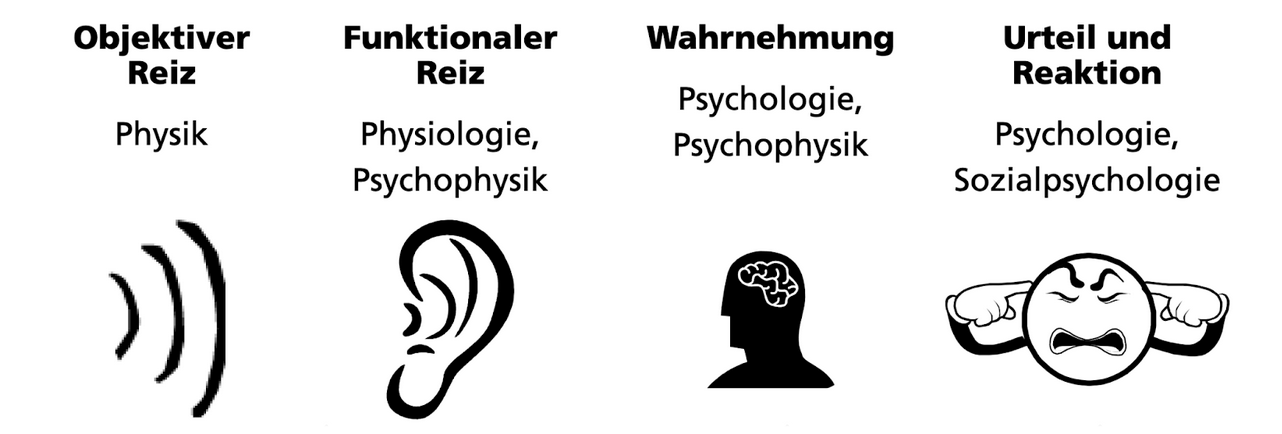
\includegraphics[width=0.8\textwidth]{bilder/fraunhofer_akustik.png}
    \caption{Akustische Reize in der Wahrnehmung (\cite{fraunhofer})}
    \label{fig10:fraunhofer}
\end{figure}\\

Die akustische Gestaltung einer Umgebung wird auch als Sounddesign oder akustische Produktgestaltung bezeichnet. Das Ziel ist dabei, ein Geräusch oder eine Geräuschkulisse zu schaffen, die den Erwartungen der Nutzer entspricht oder verkaufsfördernd wirkt. \\

\section{Emotionaler Einfluss von audiovisuellen Medien} 
Da die Wirkung von audiovisuellen Medien auf verschiedenen Ebenen der Wahrnehmung stattfindet und nicht isoliert betrachtet werden kann, hat sich die Forschungslage über die Jahre als divergent und vielschichtig herausgestellt. Der Grund für diese Diversität liegt in der inhärenten Komplexität des Untersuchungsgegenstands. 

Bereits im Jahr 2004 führten \cite{1386249} Untersuchungen durch, in denen sie mithilfe eines zweidimensionalen Modells versuchten, sowohl die Intensität der durch audiovisuelle Medien hervorgerufenen Emotion als auch deren Valenz zu messen. Unter "Valenz" versteht man allgemein die qualitative Ausrichtung einer Emotion, also ob sie als positiv oder negativ empfunden wird. Um die Intensität und die Valenz zu bestimmen, wurde der audiovisuelle Inhalt in verschiedene Komponenten zerlegt. Dabei wurden die Bewegungsmuster der aufeinanderfolgenden Einzelbilder (Frames), die Gleichmäßigkeit des Timings, der Schnitte und die Frequenzbandbreite analysiert. Bei der Auswertung der Valenz wurde hauptsächlich der Mittelwert der Tonhöhe berücksichtigt. Hierbei wurde postuliert, dass ein niedriger Mittelwert eher eine traurige Emotion, während ein hoher Mittelwert eine freudige Emotion repräsentiert. Jedoch bietet dieses Modell einen limitierten Blick auf die Emotionen, da es lediglich zwischen positiven und negativen Emotionen differenziert. 

Neuere Untersuchungen von \cite{SMALLEY2023102060} (2023) brachten weiterführende Erkenntnisse. Diese Studien konzentrierten sich auf die Betrachtung von Naturfilmen und konnten signifikante Unterschiede zwischen Versionen ohne akustische Unterstützung und solchen mit akustischer Unterstützung feststellen. Es wurde beobachtet, dass die Version mit akustischer Unterstützung eine stärkere Erregungsreaktion hervorrief und natürliche Umgebungsgeräusche Emotionen wie kognitive Erholung, Gelassenheit, Ehrfurcht und Nostalgie auslösen konnten. 

Im Kontext des digitalen Designs, insbesondere bei ausschließlich akustisch gestütztem Webdesign, gibt es Anhaltspunkte dafür, dass audiovisuelle Elemente, wie Musikvideos, ein erhöhtes Engagement beim Nutzer fördern können. Die Kombination von Interaktivität und Bewegung, zusammen mit akustischen Signalen, hat das Potenzial, den Nutzer stärker emotional zu binden.


\section{Zusammenfassung der Einflüsse} 
In der folgenden Tabelle sind (visuelle) Merkmale zusammengefasst, die auf einer Webseite eingesetzt werden können, um bestimmte emotionale Effekte bei einem Nutzer hervorzurufen. \\



\begin{center}
    \begin{tabular}{c | c | c}
%        \begin{table}
            Nr. & Merkmal                                         & Verstärkung von \\
            \hline
            1.  & Große Bilder, große Darstellung von Personen    & Erregung \\
            2.  & leuchtende Farben, hohe Sättigung               & Erregung\\
            3.  & hohe Kontraste                                  & Erregung\\
            4.  & dunkle Farben (schwarz), kühle Farben (silber)  & Dominanz\\
            5.  & eckige, gerade Formen                           & Dominanz\\
            6.  & helle, warme, klare, zarte Farben  (Gold, rosa) & Unterwürfigkeit\\
            7.  & runde, weiche, zarte Formen/Übergänge           & Unterwürfigkeit\\
%        \end{table}
    \end{tabular} \\
\end{center}

\begin{figure}[H]
    \centering
    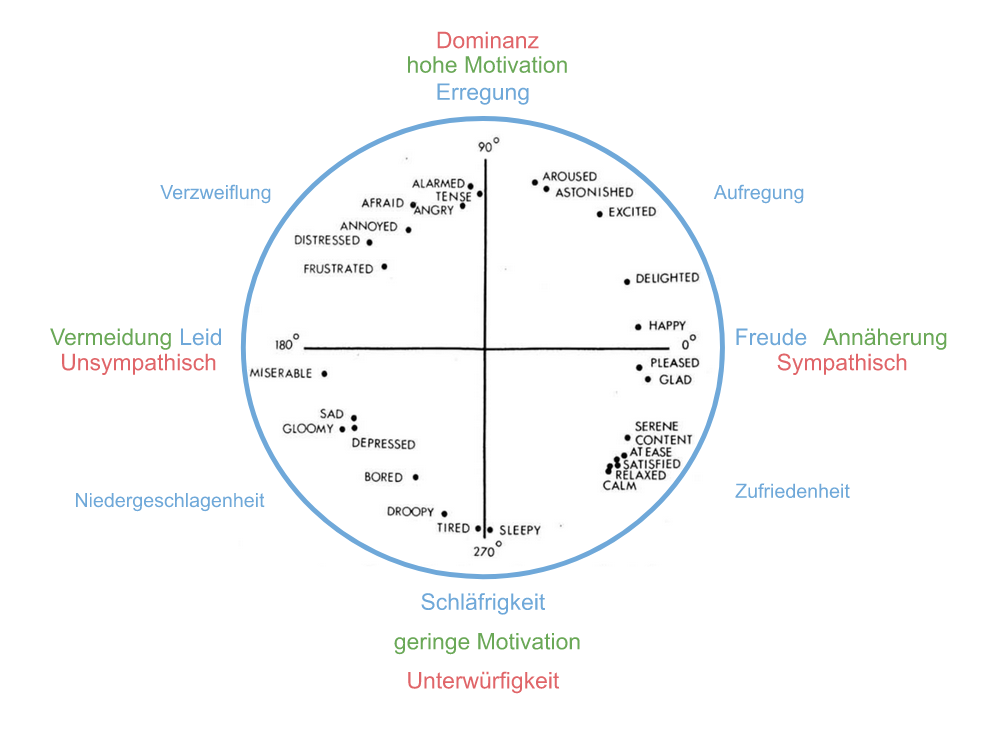
\includegraphics[width=0.8\textwidth]{bilder/dom-unt-bild.png}
    \caption{Kategorisierung unterschiedlicher Reize}
    \label{fig11:dom-unt}
\end{figure}\\

\end{document}


